%%%%%%%%%%%%%%%%%%%%%%%%%%%%%%%%%%%%%%%%%%%%%%%%%%%
%
% File: commands.tex
% 
% This file is part of the PSIThesis.cls
% LaTeX documentclass
% 
% The code in this file is made available
% under the following license:
%
% LPPL v1.3c (http://www.latex-project.org/lppl)
%
%%%%%%%%%%%%%%%%%%%%%%%%%%%%%%%%%%%%%%%%%%%%%%%%%%%


% --------------------------------------------------------
% 			CUSTOM COMMANDS FOR BETTER USABILITY
% --------------------------------------------------------


% Custom image command to insert an image
% This command uses 4 required and one optional arguments/parameters with the following meaning:
%
% Optional:
% 1 - Position of the figure (the default position is 't' for top; if no argument is provided, 't' is used
%
% Required:
% 1 - Width of the image
% 2 - Path to the image (inside the figures folder)
% 3 - Caption of the image
% 4 - Label for the image (a universal fig: is prepended)
%
% Required ----------------------------------------------------------------------------
% Optional -------------|		|			  |					|					  |
% 						V		V (1)		  V	(2)				V (3)				  V (4)
% Example Usage: \image[h]{\textwidth}{barplot-before}{This is a fancy barplot.}{barplot-before}
%
% The result will be the same as:
%
% \begin{figure}[h]
% 	\centering
% 	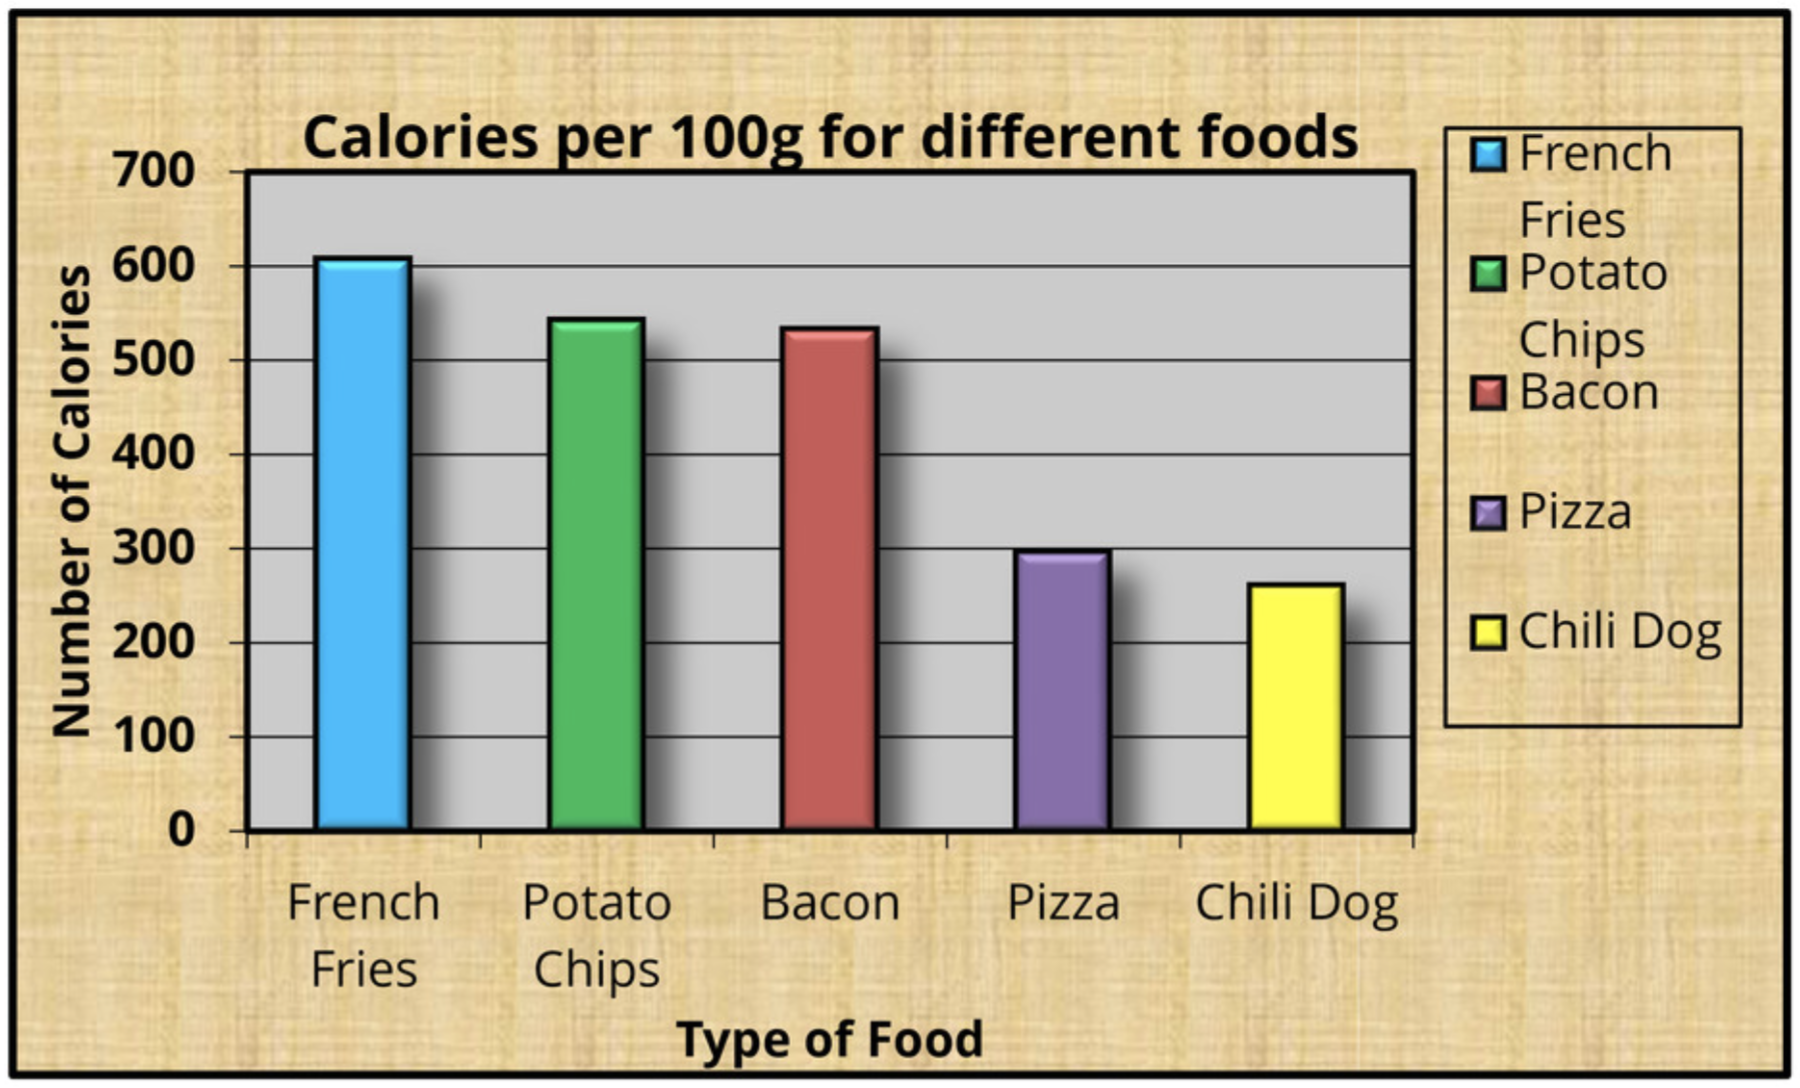
\includegraphics[width=\textwidth]{../figures/barplot-before}
% 	\caption{This is a fancy barplot.}
% 	\label{fig:barplot-before}
% \end{figure}

\newcommand{\image}[5][t]{
	\begin{figure}[#1]
		\centering
		\includegraphics[width=#2]{../figures/#3}
		\caption{#4}
		\label{fig:#5}
	\end{figure}
}

% Custom command to insert two images next to each other with a margin caption
% This command uses 6 required and one optional arguments/parameters with the following meaning:
%
% Optional:
% 1 - Position of the figure (the default position is 't' for top; if no argument is provided, 't' is used
%
% Required:
% 1 - Path to the frist image (inside the figures folder)
% 2 - Path to the second image (inside the figures folder)
% 3 - Caption of the image
% 4 - Label for the image (a universal fig: is prepended)
%
% Required --------------------------------------------------------------------------------------
% Optional -----------------|		  |			    |					|					    |
% 						    V		  V (1)		    V (2)				V (3)				    V (4)
% Example Usage: \twoimages[h]{barplot-before}{barplot-after}{This is a fancy barplot.}{barplot-sidebyside}
%
% The result will be the same as:
%
% \begin{figure}[h]
% 	\centering
% 	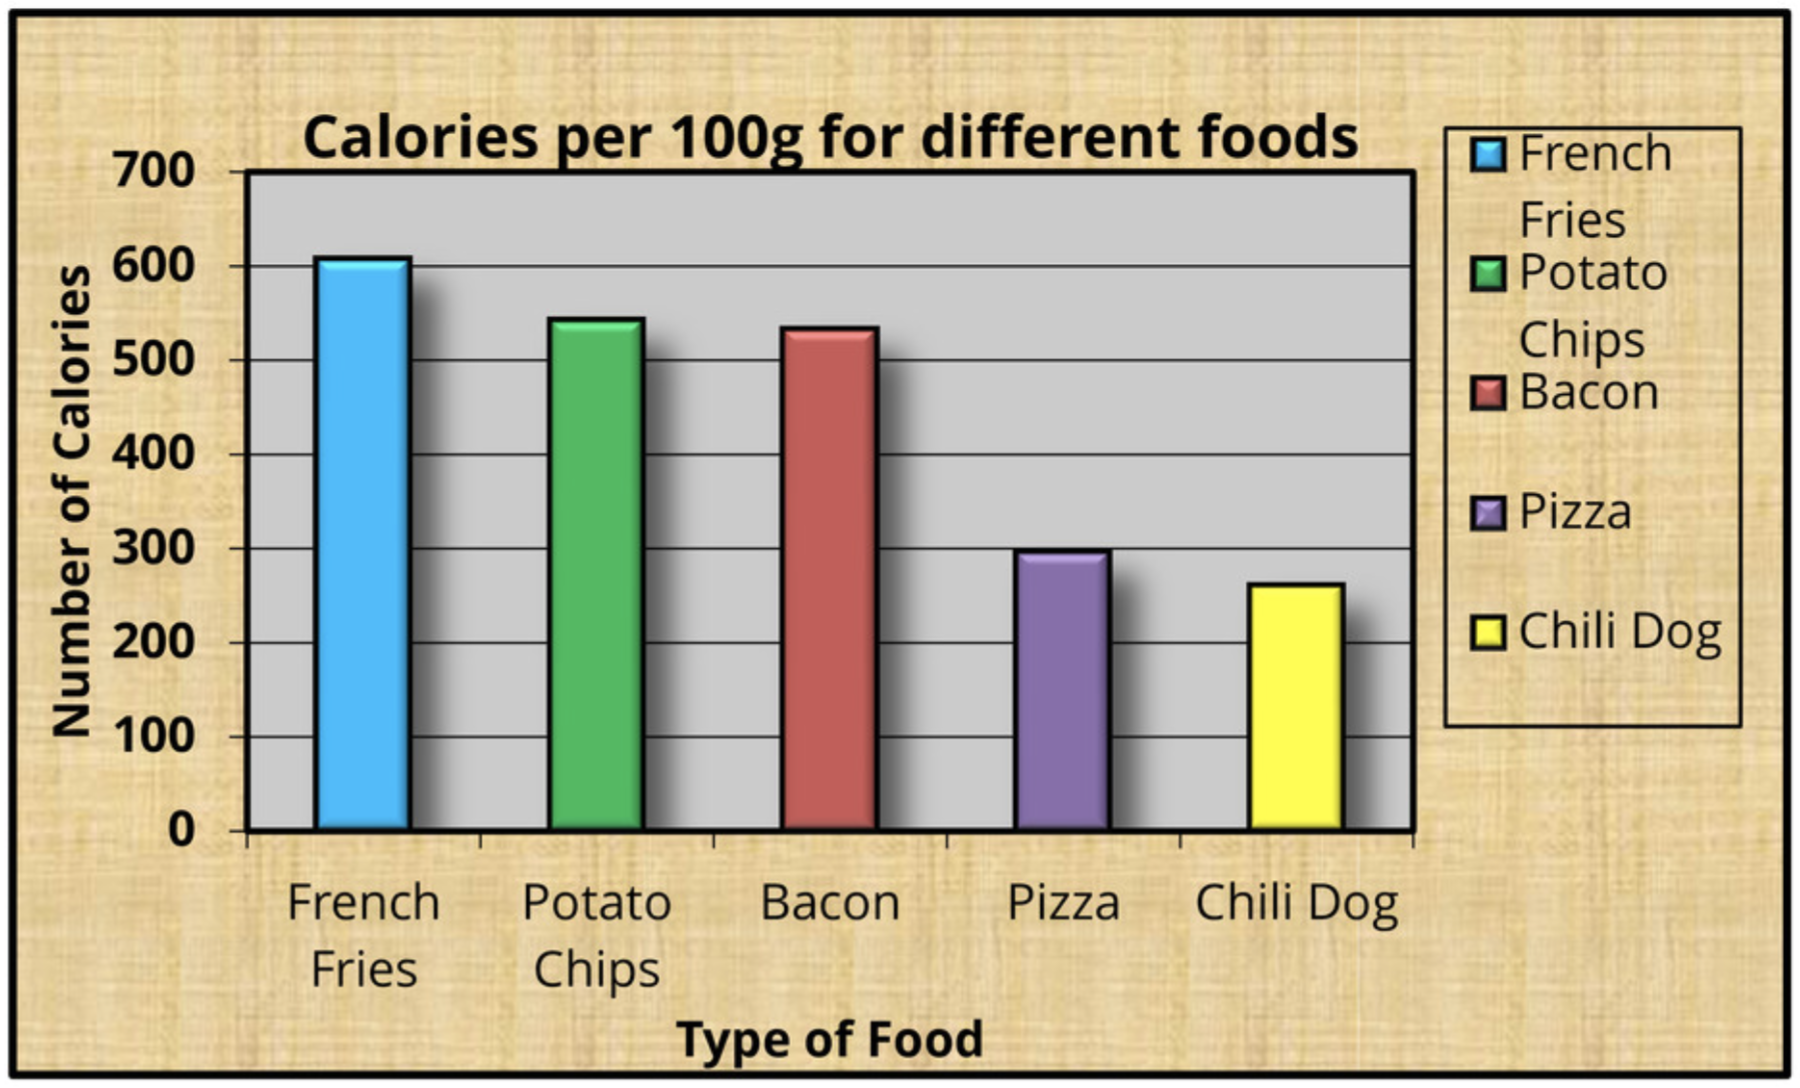
\includegraphics[width=0.48\textwidth]{../figures/barplot-before}
% 	\hspace{\fill}
% 	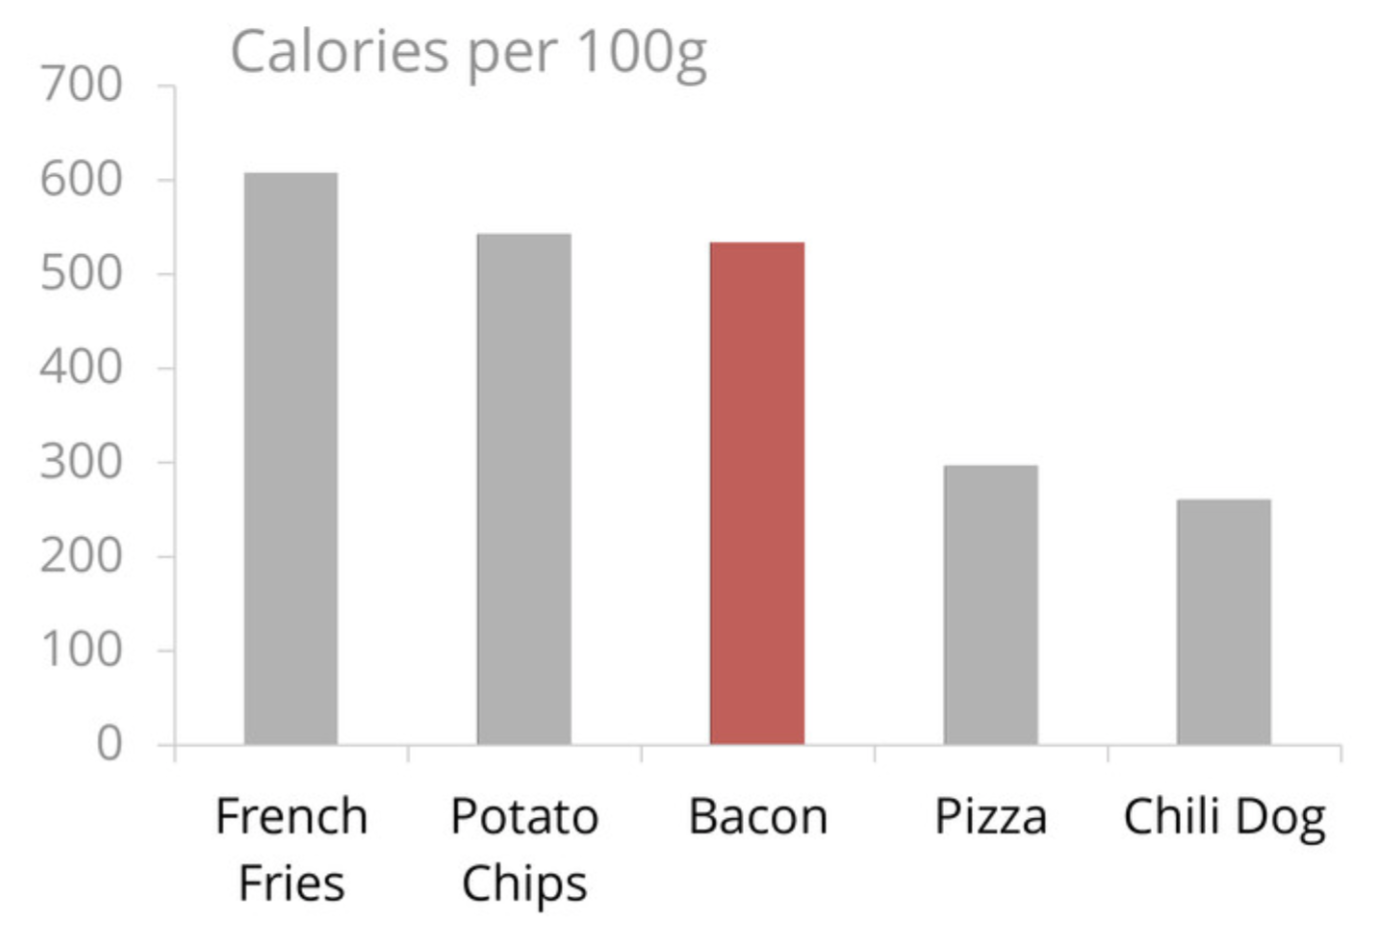
\includegraphics[width=0.48\textwidth]{../figures/barplot-after}
% 	\caption{\label{fig:barplot-sidebyside}This is a fancy barplot.}
% \end{figure}

\newcommand{\twoimages}[5][t]{
	\begin{figure}[#1]
		\centering
		\includegraphics[width=0.48\textwidth]{../figures/#2}
		\hspace{\fill}
		\includegraphics[width=0.48\textwidth]{../figures/#3}
		\sidecaption{\label{fig:#5}#4}[-2\baselineskip]
	\end{figure}
}


% Custom image command for wide figures
% This command uses 4 required and one optional arguments/parameters with the following meaning:
%
% Optional:
% 1 - Position of the figure (the default position is 't' for top; if no argument is provided, 't' is used
%
% Required:
% 1 - Path to the image (inside the figures folder)
% 2 - Caption of the image
% 3 - Label for the image (a universal fig: is prepended)
%
% Required ------------------------------------------------------------------
% Optional -----------------|		  |				 	 |					|
% 						    V		  V (1)		 	  	 V	(2)				V (3)
% Example Usage: \wideimage[h]{barplot-before}{This is a fancy barplot.}{barplot-before}
%
% The result will be the same as:
%
% \begin{figure*}[h]
% 	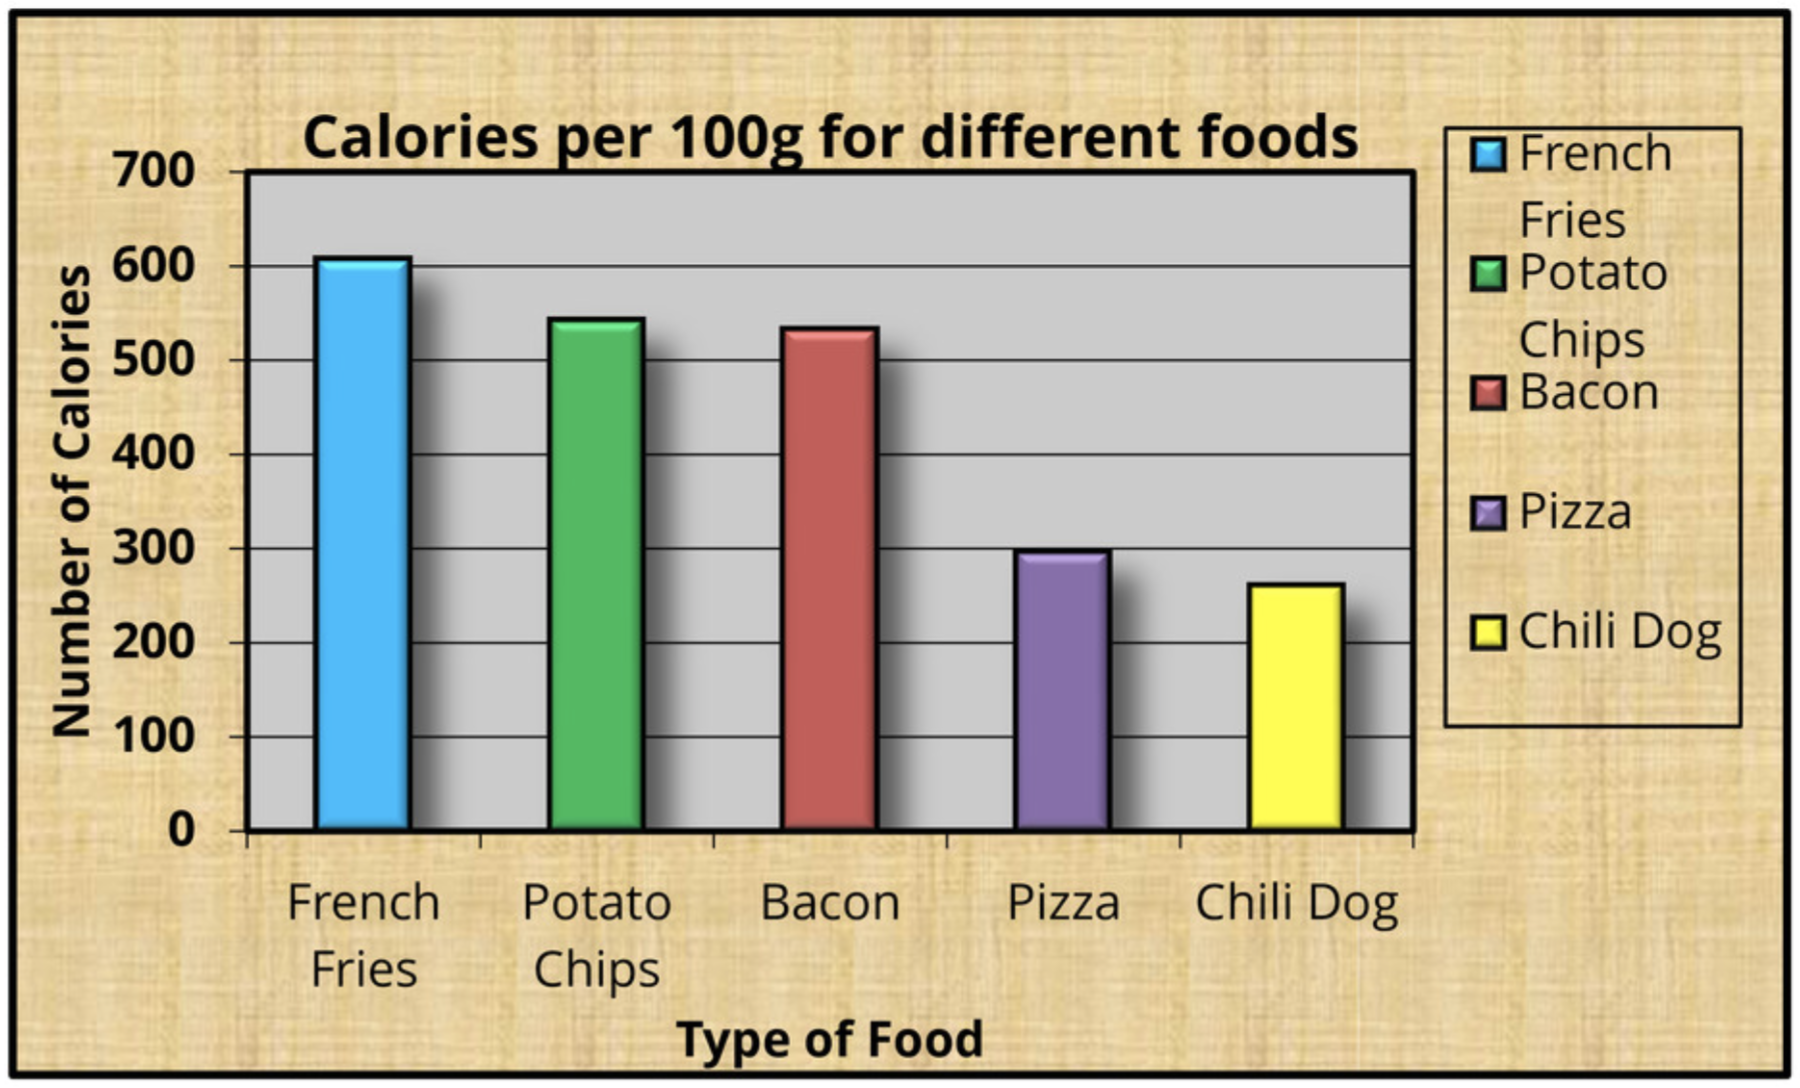
\includegraphics[width=\widefigurewidth]{../figures/barplot-before}
% 	\caption{This is a fancy barplot.}
% 	\label{fig:barplot-before}
% \end{figure*}
%
% %%%%%%%%%%%%%%%%%%%%%%%
% % 	ATTENTION		%
% %%%%%%%%%%%%%%%%%%%%%%%
% It seems this command messes with the position of other images, therefore it is advised to check the placement of other images.

\newcommand{\wideimage}[5][t]{
	\begin{figure*}[#1]
		\includegraphics[width=\widefigurewidth]{../figures/#2}
		\caption{\label{fig:#4}#3}
	\end{figure*}
}

% This command uses 3 required and one optional arguments/parameters with the following meaning:
%
% Optional:
% 1 - Vertical offset of the figure (the default offset is 1 for one line lower (negative numbers move the image up); if no argument is provided, 1 is used
%
% Required:
% 1 - Path to the image (inside the figures folder)
% 2 - Caption of the image
% 3 - Label for the image (a universal fig: is prepended)
%
% Required ----------------------------------------------------------------------
% Optional -------------------|			|				  |						|
% 							  V			V (1)			  V	(2)					V (3)
% Example Usage: \marginimage[2]{barplot-before}{This is a fancy barplot.}{barplot-before}
%
% The result will be the same as:
%
% \begin{marginfigure}[2\baselineskip]
% 	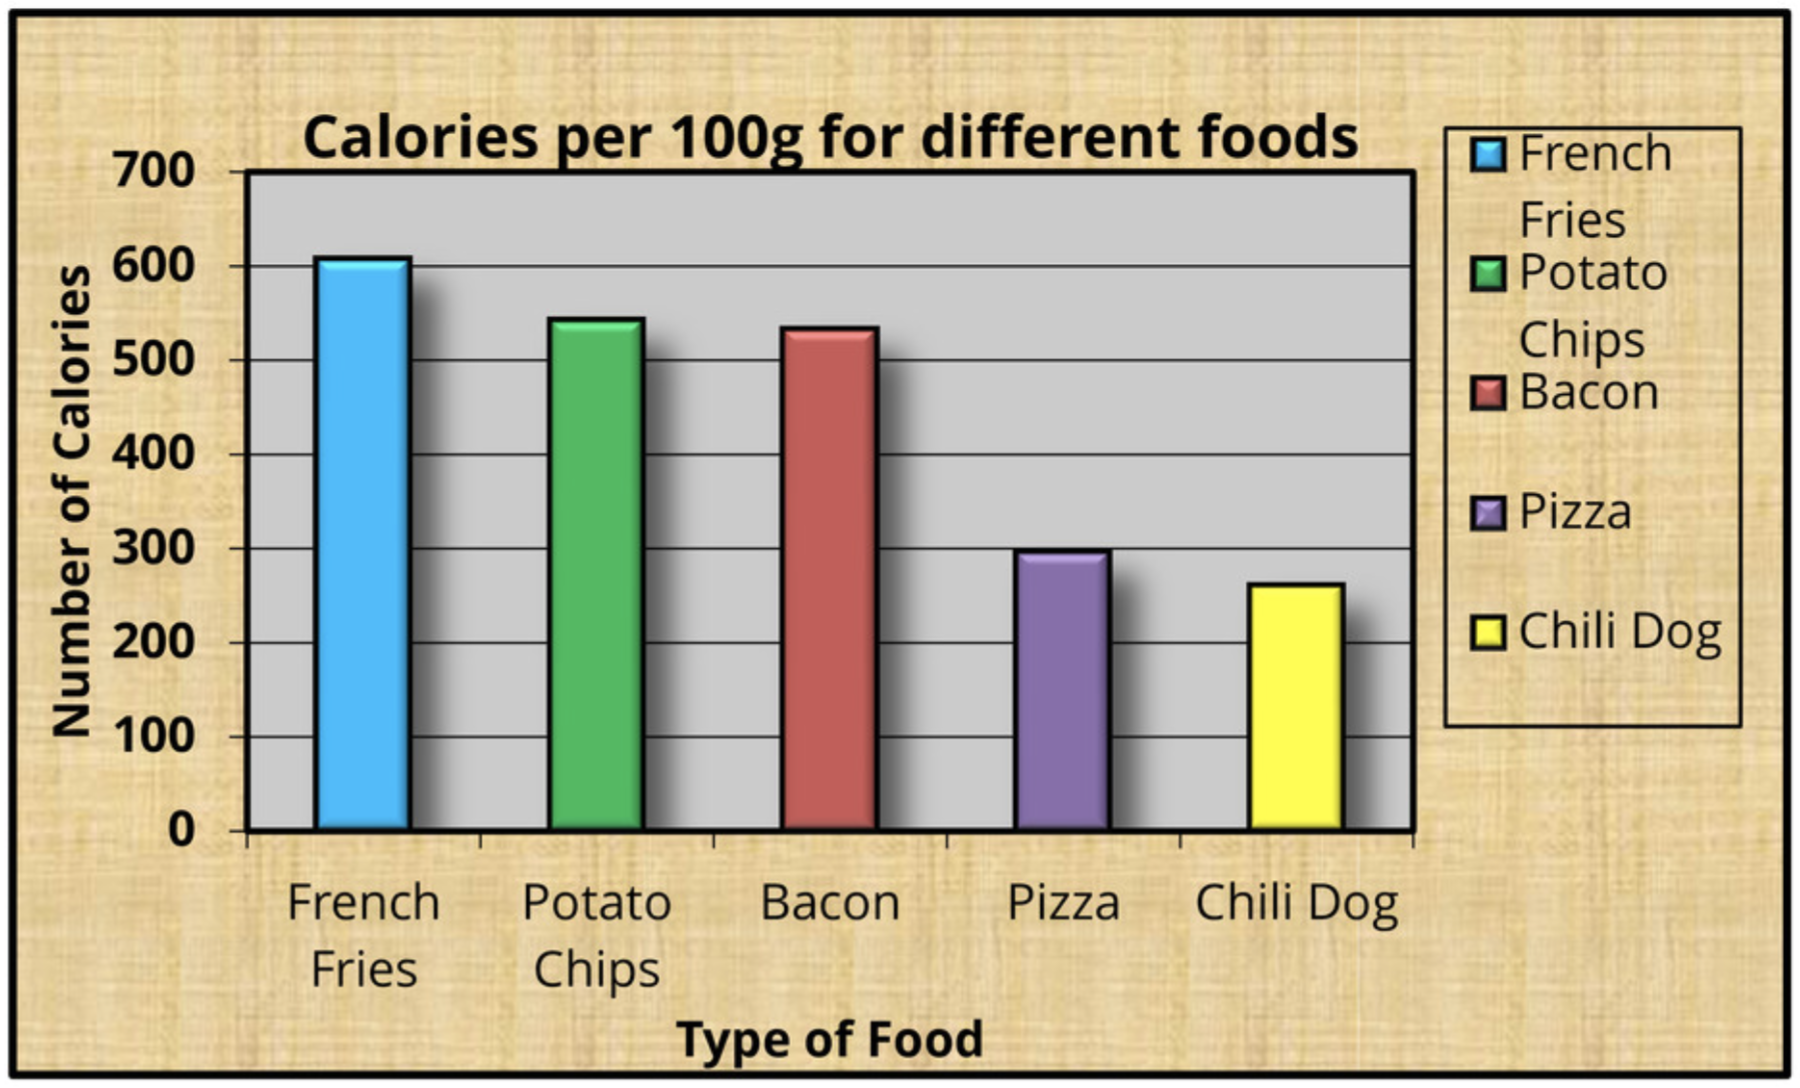
\includegraphics[width=\marginparwidth]{../figures/barplot-before}
% 	\caption{\label{fig:barplot-before}This is a fancy barplot.}
% \end{marginfigure}
\newcommand{\marginimage}[4][1]{
	\begin{marginfigure}[#1\baselineskip]
		\includegraphics[width=\marginparwidth]{../figures/#2}
		\caption{\label{fig:#4}#3}
	\end{marginfigure}
}
